\documentclass[11pt]{article}
\usepackage[margin=0.98in]{geometry}
\usepackage{amsmath,amssymb,booktabs}
\usepackage{graphicx}
\usepackage[expansion=false]{microtype}
\usepackage[font=small,labelfont=bf,skip=4pt]{caption}
\usepackage[colorlinks=true,linkcolor=black,citecolor=black,urlcolor=blue]{hyperref}
\usepackage{titlesec}
\titlespacing{\section}{0pt}{0.95em}{0.35em}
\titlespacing{\subsection}{0pt}{0.8em}{0.3em}
\setlength{\parskip}{0.22em}
\renewcommand{\topfraction}{0.92}
\renewcommand{\bottomfraction}{0.75}
\renewcommand{\textfraction}{0.06}
\renewcommand{\floatpagefraction}{0.85}
\newcommand{\rs}{$r^{*}$}

\begin{document}

\begin{center}
{\large\textbf{Whose \boldmath$r^{*}$?}}\\[0.3em]
{\normalsize Belief Transmission, Intercept Disagreement, and the Price of Long Bonds}\\[0.5em]
{\small Prospectus, short version \textperiodcentered\ 11 August 2026}
\end{center}
\vspace{0.1em}
\noindent\rule{\textwidth}{0.4pt}
\suppressfloats[t]

\vspace{0.2em}
{\footnotesize\noindent Condensed from the full v2 prospectus, which carries the derivations,
the qualifications to each test, and the full positioning discussion.}

% =====================================================================
\section{The question}

The federal funds rate is an overnight rate. The ten-year Treasury yield is not, and its
thirty-year decline is usually attributed to forces outside monetary policy. Hillenbrand
(2025) shows that the decline accumulated almost entirely inside three-day windows around FOMC
announcements, and argues the Fed was revealing its own estimate of the long-run equilibrium
rate.

That interpretation makes a structural claim nobody has examined. Writing the policy rule as
\begin{equation}
i_t \;=\; \underbrace{r^{*}_t + \pi^{*}_t}_{\text{intercept}} \;+\; \phi_\pi\!\left(\pi_t - \pi^{*}_t\right) + \phi_x x_t + v_t ,
\label{eq:rule}
\end{equation}
\rs{} is the \emph{intercept} of the reaction function, so ``the Fed reveals \rs{}'' means the
Fed is telling markets about the constant in its own rule. Bauer, Pflueger \& Sunderam (2024)
estimate the perceived \emph{slope} $\phi_\pi$ and show it prices term premia; they absorb the
intercept into forecaster fixed effects and say so explicitly. The intercept has been assumed
known, assumed common, or differenced away.

\begin{quote}
\textbf{How does the Fed move beliefs about the intercept of its own reaction function, and
what does disagreement about that intercept do to the price of long bonds?}
\end{quote}

\noindent In three parts: \textbf{(1) transmission} --- does the published longer-run
projection move market beliefs, and in which direction does causality run; \textbf{(2)
pricing} --- does the belief revision reach long yields with the maturity signature of an
endpoint shock rather than a stance shock; \textbf{(3) disagreement} --- is uncertainty about
the intercept compensated in the term premium, asymmetrically in the sign of the perceived
error?

\subsection*{What the data have already removed}

Three results below constrain this severely, and it is better to say so at the front. Fact 3
shows the yield response to be explained is concentrated \emph{before} the published projection
exists. Fact 2 shows the signed Fed-minus-market gap has a standard deviation of 10 bp. \S6.4
shows neither candidate market-side \rs{} measure is usable. So Part 1 is estimated where the
yield response is indistinguishable from zero and is informative mainly as a null; the
dispersion half of Part 3 is Cao, Crump, Eusepi \& Moench (SR 934) with a different dispersion
series and the signed half has no usable post-2012 variation; and \textbf{Part 2 --- the
maturity signature with its nominal/TIPS split --- is the one element that has power on
assembled data, can fail, and is not occupied}. The prospectus is organised around it. A
second, independent component (\S5) requires none of these assumptions.

% =====================================================================
\section{Three facts}

Established on assembled data: GSW zero-coupon yields, the ACM daily decomposition, a
hand-built FOMC calendar of 300 scheduled meetings and 73 unscheduled actions covering June
1989 -- July 2026, the SEP dot-plot archive from 2012, and the NY Fed Survey of Primary Dealers
longer-run funds rate from 2013.

\subsection{Fact 1: long yields fall only when the Fed is in the room}

June 1989 -- June 2021: the ten-year fell 6.99 pp, of which 6.16 pp (88\%) accrued in three-day
FOMC windows representing 11.8\% of trading days. Outside, the drift is $-0.012$ bp/day
($t=-0.18$) over 7{,}035 days; a randomisation test places the observed figure at the 0th
percentile of 5{,}000 draws.

This is a statement about \emph{conditional means by day type}, not about the permanence of
innovations: the two day types have nearly identical daily volatility (6.72 versus 5.60 bp).
What distinguishes announcement days is that news arriving on them has carried a systematically
negative sign for three decades. Extending to July 2026 constrains any mechanism: over
2022--2026 the Fed raised the target 525 bp and the ten-year rose 2.60 pp, but in FOMC windows
it \emph{fell} 1.20 pp --- the entire tightening happened on non-FOMC days
(Figure~\ref{fig:fact}).

\begin{figure}[tbp]
\centering
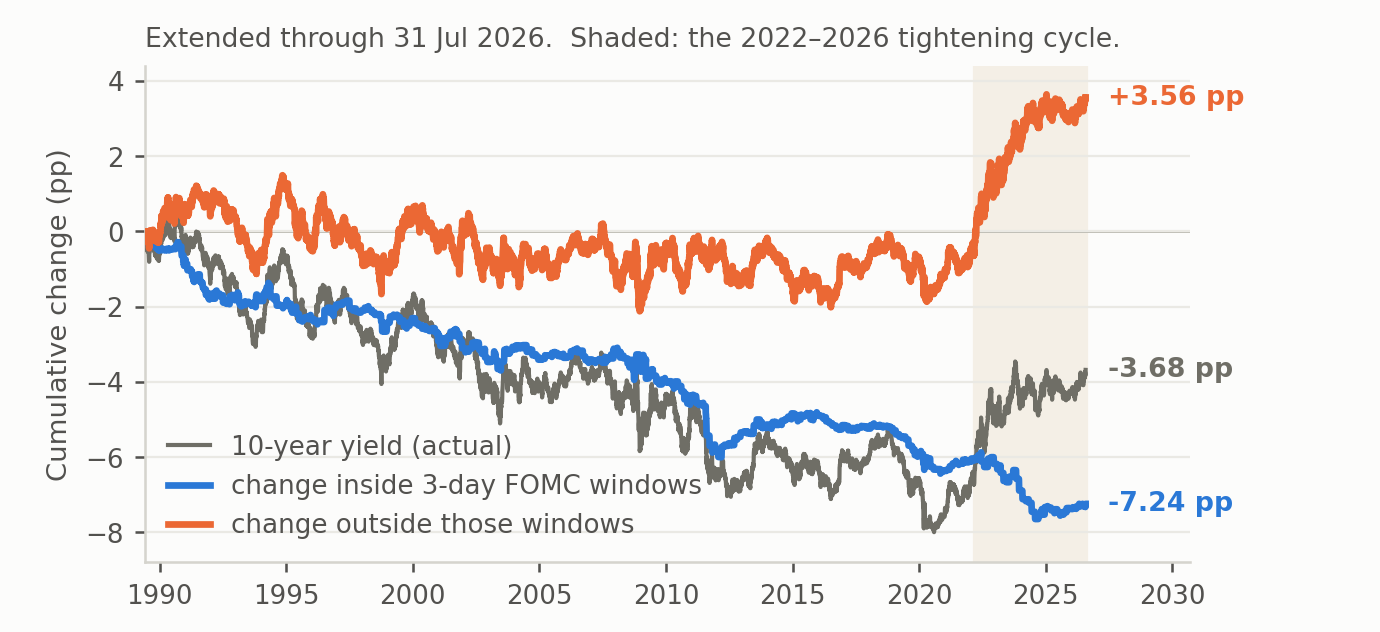
\includegraphics[width=0.78\textwidth]{s_extend.png}
\caption{\textbf{Fact 1.} Cumulative change in the ten-year yield from 2 June 1989, split into
the part accruing inside three-day FOMC windows and the part accruing on all other days.
Shaded: the 2022--2026 tightening cycle.}
\label{fig:fact}
\end{figure}

\subsection{Fact 2: the two beliefs move together, and asymmetrically}

The FOMC publishes its longer-run funds rate projection quarterly; the NY Fed surveys primary
dealers for the same object about two weeks before every meeting. Netting the 2\% objective
from both gives two comparable measures of \rs{} with no term-structure model anywhere
(Figure~\ref{fig:beliefs}). Across 48 matched meetings: the gap has a standard deviation of
0.105 pp and a range of $-0.11$ to $+0.30$, exceeding 25 bp at 4\% of meetings; dealers move
with the Fed nearly one-for-one ($\beta = 0.82$, $t=6.86$); the reverse relation is present but
weaker ($\beta = 0.31$, $t=3.91$).

\begin{figure}[tbp]
\centering
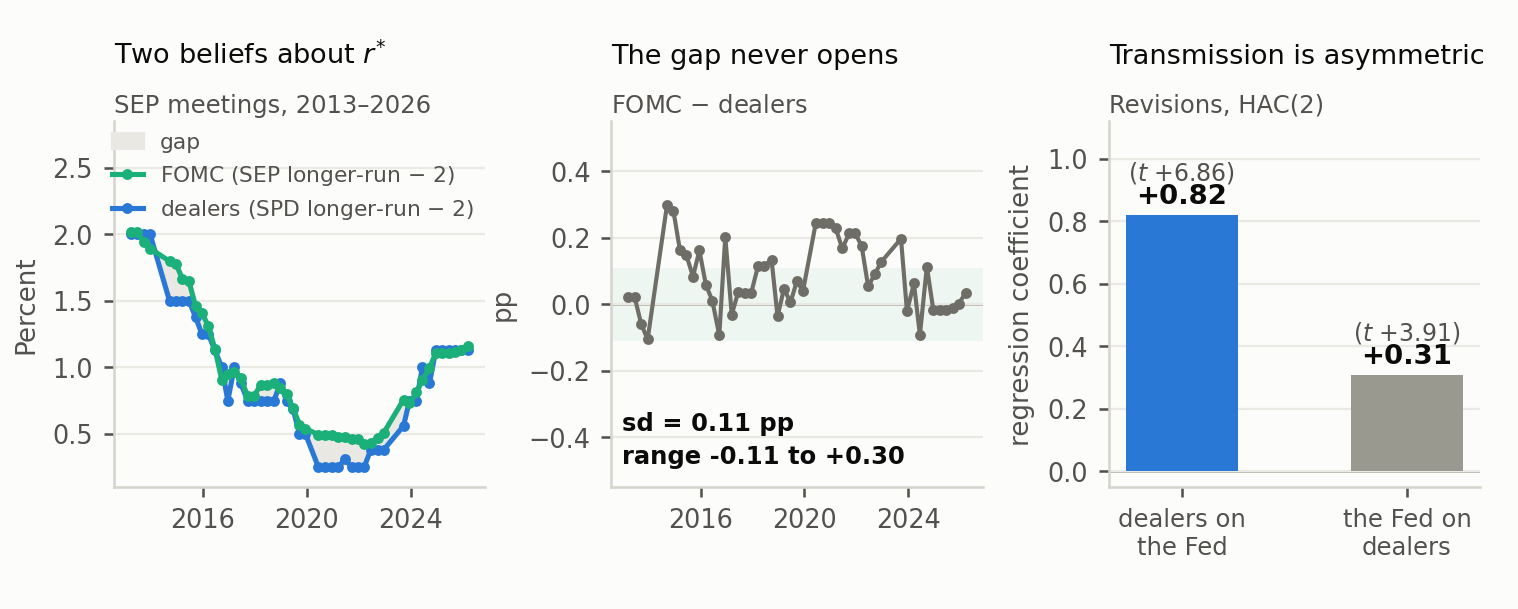
\includegraphics[width=0.82\textwidth]{s_beliefs.png}
\caption{\textbf{Fact 2.} Left: the FOMC's longer-run projection and the primary dealers'
longer-run funds rate, each less 2.0. Centre: the difference. Right: revision regressions,
HAC(2), 46--47 meetings.}
\label{fig:beliefs}
\end{figure}

The asymmetry is not mechanical --- the Desk briefs the FOMC with survey results before each
meeting --- but it is not a clean lead-lag either. In a horse race the dealer revision loads on
both the preceding dot revision (0.60) and the contemporaneous one (0.58), so part of what looks
like following is anticipation. Both series are observed eight times a year, and the
simultaneity cannot be resolved within them by any market-price measurement.

\subsection{Fact 3: the phenomenon predates the measure}

\begin{center}\small
\begin{tabular}{lrrr}
\toprule
Period & bp/meeting & $t$ & Cumulative\\ \midrule
Jun 1989 -- Dec 2011 (pre-SEP) & $-2.46$ & $-3.06$ & $\mathbf{-5.85}$ pp\\
Jan 2012 -- Mar 2022 (dot falling 1.78 pp) & $-0.40$ & $-0.41$ & $-0.23$ pp\\
Mar 2022 -- Jul 2026 (dot rising 0.74 pp) & $-3.49$ & $-1.53$ & $-1.16$ pp\\
\bottomrule\end{tabular}
\end{center}

\noindent 81\% of the in-window decline is complete before the dot plot begins. In the decade
when the FOMC cut its own longer-run rate by 1.78 pp --- when an information channel should be
loudest --- the in-window contribution is indistinguishable from zero. Every design using the
published projection is therefore estimated on a sample in which the motivating phenomenon is
absent. That is an argument about the whole of Component A, not one contingency within it.

% =====================================================================
\section{Framework}

Define $i^{*}_t \equiv r^{*}_t + \pi^{*}_t$ and $\text{gap}_t \equiv i_t - i^{*}_t$, the stance
of policy. From the definition of a long yield as an average of expected short rates plus a
residual, and assuming the endpoints are locally martingales,
\begin{equation}
\Delta y^{(n)}_t \;=\; \underbrace{\Delta r^{*}_t + \Delta \pi^{*}_t}_{\text{endpoint news}}
\;+\; \underbrace{\omega(\rho,n)\,\Delta\text{gap}_t + \text{gap}_t\,\Delta\omega}_{\text{stance and persistence news}}
\;+\; \Delta TP^{(n)}_t ,
\qquad \omega(\rho,n) = \frac{1-\rho^{n}}{n(1-\rho)} .
\label{eq:windowdiff}
\end{equation}
Four terms, one observable. Reading window moves as endpoint news requires three separate
exclusions. The stance exclusion is defended by noting the pattern survives in the 5y5y forward,
where the analogous weight
$\omega^{f} = \rho^{n_1}(1-\rho^{n_2})/[n_2(1-\rho)]$ is small --- but how small is an empirical
question about $\rho$:

\begin{center}\small
\begin{tabular}{lcccc}
\toprule
Half-life of the gap & $\omega$, 2-year & $\omega$, 5-year & $\omega$, 10-year & $\omega^{f}$, 5y5y\\ \midrule
1 year  & 0.56 & 0.29 & 0.15 & 0.01\\
2 years & 0.73 & 0.48 & 0.28 & 0.09\\
4 years & 0.85 & 0.67 & 0.48 & 0.28\\
\bottomrule\end{tabular}
\end{center}

\noindent An AR(1) on a crude gap proxy --- the one-year yield less HLW \rs{} plus 2 --- gives a
half-life of 4.4 years on the full sample and 4.1 post-1995. At that persistence a 100 bp stance
revision moves the ten-year about 50 bp and the 5y5y forward about 30 bp, so the far-forward
evidence does not by itself separate endpoint news from stance news.

\subsection{The maturity signature, and what it can and cannot separate}

Endpoint news enters $y^{(n)}$ with a coefficient of one at every maturity; stance news enters
with $\omega(\rho,n)$, strictly decreasing in $n$. So the \emph{shape} of the window response
across maturities discriminates, with a slope pinned down by $\rho$. Three qualifications
belong in the statement of the test, not in a robustness appendix.

\emph{The martingale assumption is load-bearing.} Endpoint news is flat only because $r^{*}$
and $\pi^{*}$ are assumed martingales. If perceived \rs{} revisions are partly transitory ---
which learning models allow --- endpoint news also enters as $\omega(\rho^{*},n)$ with
$\rho^{*}$ near one, and the test discriminates two decay rates rather than flat against
declining.

\emph{This is close to a factor decomposition.} Over 2--10 years, flat is approximately level
and declining approximately slope, so the raw test asks what Gürkaynak, Sack \& Swanson (2005)
and Swanson (2021) have asked for twenty years. The contribution is the \emph{restriction}:
$\omega(\rho,n)$ is a one-parameter family, $\rho$ is estimable outside the event sample, and
the over-identifying content is whether the $\rho$ fitting the maturity profile matches the
$\rho$ fitting the gap dynamics.

\emph{The TIPS split is what makes it sharp.} $\Delta TP^{(n)}$ has an unrestricted maturity
profile, so any shape can in principle be rationalised as a premium response; the test is
informative conditional on that response being smooth. Running the same test on the real curve
removes $\Delta\pi^{*}$ entirely, and the nominal-minus-real difference identifies the
inflation-expectation component directly. That comparison, not the nominal shape alone, is the
element with no close antecedent.

\subsection{Two channels, kept distinct}

\textbf{Channel 1, a disagreement premium} in $\sigma^2_{\delta}$: dispersion about the intercept
propagates into the variance of the whole expected path, undamped by horizon, so the predicted
term-premium sensitivity rises with maturity and does not decay. This differentiates the project
from Caballero \& Simsek, whose demand disagreement mean-reverts --- and it is also what Cao
et al.\ substantially occupy.

\textbf{Channel 2, a level effect of the signed gap} $\delta \equiv r^{*m} - r^{*F}$: the market
evaluates the stance against its own neutral rate while the Fed sets policy against its own.
Positive $\delta$ means policy looks too easy --- expected overshoot, an expected correction,
compensation in the inflation dimension; negative $\delta$ the reverse. This object is
\emph{transitory}, so its yield effect is hump-shaped in maturity, not flat. The defence against Caballero \& Simsek
applies to Channel 1 only, and that is the channel Cao et al.\ occupy.

Writing the investor's expected path with the Fed's intercept but his own read of the stance,
\begin{equation}
y^{(n)}_t \;=\; \underbrace{r^{*F}_t + \pi^{*}_t}_{\text{endpoint}} + \underbrace{\omega(\rho,n)\,\text{gap}_t}_{\text{stance}} + \underbrace{\Lambda(n)\,\delta_t}_{\text{perceived error}} + \underbrace{TP^{(n)}\!\left(\sigma^2_{\delta,t}\right)}_{\text{disagreement premium}} .
\label{eq:pricing}
\end{equation}
Two caveats stated as such. The long-run anchor here is $r^{*F}$, the \emph{Fed's} estimate,
whether or not it is correct --- a strong assumption, and the opposite of the accounting
argument that the Fed cannot durably move \rs{}; an anchor
$\theta r^{*F} + (1-\theta)r^{*m}$ nests both and makes $\theta$ estimable from the maturity
profile. And $\Lambda(n)$'s hump shape is currently imposed rather than derived, so as written
the hump prediction cannot fail; deriving $\lambda_j$ from a stated Phillips curve and rule,
which pins down the peak location, is scheduled work.

What does come free is the sign split: $\delta$ enters expected inflation and the expected real
path with opposite signs, so the division of the response between the nominal and TIPS curves
identifies the sign channel with no decomposition of the nominal curve.

% =====================================================================
\section{Position in the literature}

\begin{center}\footnotesize
\begin{tabular}{@{}p{0.27\textwidth}p{0.31\textwidth}p{0.35\textwidth}@{}}
\toprule
\textbf{Paper} & \textbf{Object} & \textbf{What it leaves open}\\ \midrule
Hillenbrand (2025, \emph{RFS}) & Window decline is endpoint learning & Never tests the exclusions; no belief data\\[0.25em]
Gürkaynak, Sack \& Swanson (2005); Swanson (2021) & Target/path/LSAP factors from the cross-maturity response & Statistical factors; no restriction tying the loading to an estimated $\rho$\\[0.25em]
Bauer, Pflueger \& Sunderam (2024, \emph{QJE}) & Perceived \emph{slope} $\phi_\pi$; prices term premia & Absorbs the intercept into forecaster fixed effects, explicitly\\[0.25em]
Cao, Crump, Eusepi \& Moench (SR 934) & Forecaster disagreement about the long-run level; $\sim$1/3 of TP variation & Unsigned; not Fed-vs-market. \emph{Occupies Channel 1}\\[0.25em]
Caballero \& Simsek (2022, \emph{AER}) & Fed-market disagreement $\to$ sign-dependent policy risk premium & Disagreement is about \emph{demand}, which mean-reverts; no term structure, no TIPS\\[0.25em]
Cieslak \& McMahon; Cieslak, McMahon \& Pang & Perceived policy errors raise term premia & Error is about the state and the slope, never the intercept\\[0.25em]
Savor \& Wilson; Ai \& Bansal; Lucca \& Moench & Announcement-day risk premia in bonds & A \emph{return} premium needing no offset; silent on the sign of the yield change. Central to \S5\\
\bottomrule\end{tabular}
\end{center}

\vspace{0.3em}
\noindent Unclaimed: disagreement that is Fed-versus-market rather than
forecaster-versus-forecaster; a \emph{signed} gap rather than dispersion; and the mapping from
sign to \emph{which} risk is compensated. The SEP \emph{longer-run} dot as an asset-price
regressor is also effectively unused. But the differentiated space is narrower than that list
suggests: the Caballero--Simsek defence applies only to the channel Cao et al.\ occupy, and
Gürkaynak--Sack--Swanson is why \S3.1 must be presented as a restricted shape test rather than a
new design. Note also that the rule framing is not doing all the work it appears to: every
loading in \eqref{eq:pricing} follows from ``there is a long-run anchor and agents disagree about
it,'' and since all archived longer-run PCE submissions are exactly 2.0, intercept disagreement
reduces empirically to disagreement about the longer-run nominal dot. The framing earns its place
by making the differentiation from Bauer--Pflueger--Sunderam precise: same rule, different
coefficient.

% =====================================================================
\section{Component A: transmission and pricing}

\textbf{A1. Does the projection move prices?} The longer-run dot is published at four meetings a
year and not the other four, giving a within-Fed contrast that holds announcement format fixed:
\begin{equation}
\Delta y^{(n)}_t = \alpha + \beta_1 \text{SEP}_t + \beta_2 \left(\text{SEP}_t \times |\Delta \text{dot}^{LR}_t|\right) + \gamma' Z_t + \varepsilon_t ,
\label{eq:sep}
\end{equation}
with $Z_t$ containing the Kuttner (2001) surprise, the path factor, and pre-meeting controls in
the spirit of Bauer \& Swanson (2023). The minimum detectable effect is computed and reported
\emph{before} estimation --- 57 meetings, roughly 28 with a non-zero revision, residual window
standard deviation about 7 bp --- so that a null is interpretable. Note that intraday data does
not help identify this: the SEP arrives at 2:00 pm in the same tick as the statement and the
near-term dots, so intraday windows separate statement-plus-SEP from press conference and nothing
finer.

\textbf{A2. The maturity signature \emph{(core test)}.} Estimate the window response at every GSW
maturity from 1 to 30 years on meetings where the longer-run projection was revised, and test the
restriction in \S3.1 with $\rho$ first fixed at its gap-process value and then free; the
over-identifying test is whether the two agree. Repeat on the TIPS curve and report the
nominal-minus-real difference. Report the estimated profile alongside the first two principal
components over the same grid, so the reader can see how much of the result is level-versus-slope
and how much is the restriction.

\textbf{A3. Is intercept disagreement priced? \emph{(bounded)}} Dispersion varies usefully where
the level gap does not: the dealer interquartile range spans 0--0.75 pp and the FOMC's own
cross-participant standard deviation 0.22--0.46 pp. Regress long-horizon forward term premia on
intercept dispersion, orthogonalised against the Bauer--Lakdawala--Mueller option-implied
uncertainty measure and against Cao et al.'s forecaster dispersion; the coefficient of interest
is what survives that control. The only element not already claimed is the prediction that the
sensitivity does not decay with maturity.

\textbf{A4. Asymmetry in the sign \emph{(contingent)}.} Fact 2 rules out the simplest version.
Three routes, in descending confidence: the pre-2012 Tealbook sample against contemporaneous Blue
Chip long-range forecasts, where level disagreement is plausible and the yield response lives;
distributional rather than median gaps, since tail disagreement may be larger even when medians
coincide; and revision direction rather than level, which with 18 upward revisions gives 21--31\%
power. If the first two fail, A4 is dropped.

% =====================================================================
\section{Component B: why announcement-day news has one sign}

Component A rests on a chain of maintained assumptions. Component B rests on almost none.

An earlier draft framed this as ``why do only scheduled-date changes persist?'' That is not what
Fact 1 establishes. Fact 1 compares conditional means by day type; a driftless random walk has
fully permanent innovations and cumulates to zero, so permanence and drift are different objects.
The puzzle is \textbf{one-sidedness}: why has news arriving on 12\% of trading days carried a
systematically negative sign for three decades, when those days are no more volatile than any
other? That connects directly to Savor \& Wilson, Ai \& Bansal and Lucca \& Moench, who document
that bonds earn a disproportionate share of their excess return on announcement days. Their
object is a \emph{return} premium, requiring no offset and implying nothing about the sign of the
yield-level change; Hillenbrand's is a cumulating \emph{yield-level} effect, coherent only if the
yield is non-stationary over the sample. Reconciling them is the contribution, and the 2022--2026
reversal of the outside-window series to $+3.56$ pp is the first evidence the offset arrives.

Three designs. \emph{Event-time conditional mean path}: the mean daily change at each event time
from $t-10$ to $t+10$, with block-bootstrapped bands --- not done for US Treasuries, and the
shape discriminates build-then-resolve from drop-then-rebuild. \emph{Variance ratio by day type}:
a distinct object with a distinct target, adjudicating Hanson, Lucca \& Wright against
Hillenbrand; it does not test Fact 1. \emph{Stationarity accounting}: report the offset by
sub-period.

The competing explanation is Lou, Pintér, Üslü \& Walker (BIS WP 1232), who report the effect
concentrates in windows \emph{without} long-dated Treasury issuance --- dealer inventory rather
than monetary policy. This test is cheap but not decisive: Treasury issues on a fixed monthly
refunding cycle, so overlap with the FOMC calendar is mechanical and correlated with data-release
timing. Step one is counting how many of the 373 windows contain long-dated issuance and checking
whether the split is balanced; if not, the result is a control rather than an adjudication.

% =====================================================================
\section{Completed work}

\begin{enumerate}\setlength\itemsep{0.15em}
\item \textbf{The literature's disagreement about the channel is an event-list artifact.} Pan \&
Peng's day-$(t-1)$ estimates reproduce to three coefficients ($-0.785$ / $-0.716$ / $-0.070$
against $-0.79$ / $-0.71$ / $-0.08$), but the term-premium share moves from 91\% to 46\% on the
same day, same data and same decomposition, purely by changing the event list. The 73 unscheduled
actions a scheduled-only filter removes carry $-2.5$ bp of expectations decline per event against
$-0.07$ for scheduled meetings. Neither paper discusses the event list.
\item \textbf{The standard decomposition cannot arbitrate.} $\Delta rn^{(n)}_t = c_n'\Delta
y^{\mathcal N}_t$ with $R^2 = 1.00000$ over 9{,}282 daily observations, so
$\beta^{rn} = c'\beta^{\mathcal N}$ exactly and the decomposition adds no event-specific
information; $c'\mathbf 1 = 0.529$, so a permanent credible parallel shift is reported as 53/47.
Before write-up this needs the Kim--Wright figure and an explicit scope limitation to
\emph{spanned} models.
\item \textbf{The effect and the measurement do not overlap in time} --- Fact 3.
\item \textbf{Neither candidate market-side \rs{} measure is usable.} The ACM 9y1y forward loads
0.287 on the one-year yield ($R^2 = 0.83$) --- circular with yields; the survey measure has
dealers loading 0.82 on the Fed's own revision --- circular with the Fed. This closes the wedge
design rather than leaving it open.
\end{enumerate}

% =====================================================================
\section{Risks, timeline, requests}

\textbf{What would kill each component.} \emph{Power and the Tealbook dependency}: Tealbook is not
a contingency for A4, it is the only sample in which any projection-based design is estimated on
the period containing the phenomenon; without archive access Component A reduces to A2 on a weak
sample plus a null, and Component B becomes the dissertation. \emph{The maturity test may not
separate}: if the endpoint is not a martingale the test discriminates two decay rates, and 28
revisions may not distinguish them. \emph{Simultaneity is not resolved by intraday data}: Fact 2
may remain a descriptive asymmetry. \emph{Positioning}: if Caballero \& Simsek's empirics already
use the longer-run dot --- unverified --- the contribution narrows to the maturity signature and
the TIPS asymmetry.

\begin{center}\small
\begin{tabular}{@{}llp{0.55\textwidth}@{}}
\toprule
\textbf{Period} & \textbf{Component} & \textbf{Task}\\ \midrule
Weeks 1--4 & --- & Draft the reconciliation note (\S6.1--\S6.2), after adding the Kim--Wright figure and the unspanned caveat\\
Weeks 2--8 & B & Issuance-overlap count, then the event-time conditional mean path with bootstrapped bands\\
Weeks 4--6 & A & Derive $\lambda_j$; compute and report the A1 minimum detectable effect\\
Weeks 6--14 & A2 & Maturity-signature test on nominal and TIPS curves, with the PC benchmark\\
Term 2 & B, A3 & Variance ratio and stationarity accounting; dispersion and term premia\\
Contingent & A4 & Tealbook and Blue Chip, subject to access\\
\bottomrule\end{tabular}
\end{center}

\textbf{Requests.} \emph{(i)} Whether the reconciliation goes out as a standalone short piece or
becomes a methodological section, and whether the two scope caveats suffice. \emph{(ii)} Tealbook
and Blue Chip access --- these bind on the whole of Component A, not A4 alone, and this is the
highest-value resource request here. \emph{(iii)} Structure: my inclination is to lead with the
note, make Component B the first chapter respecified around one-sidedness, and fold A2 into it as
the section asking whether the one-sided announcement news is endpoint news --- one paper with a
fact, a test and a mechanism rather than two half-chapters, with A1, A3 and A4 a second chapter
conditional on Tealbook. Does that concede too much of Component A, given it is the part with the
genuinely open position?

\enlargethispage{3\baselineskip}
\vspace{0.35em}
\noindent\rule{\textwidth}{0.4pt}\\[0.2em]
\scriptsize\textbf{Key references.} Bauer, Pflueger \& Sunderam (2024), \emph{QJE}. Bauer \&
Rudebusch (2020), \emph{AER}. Caballero \& Simsek (2022), \emph{AER}. Cao, Crump, Eusepi \&
Moench, FRBNY SR 934. Gürkaynak, Sack \& Swanson (2005). Hanson, Lucca \& Wright (2021),
\emph{QJE}. Hillenbrand (2025), \emph{RFS}. Joslin, Singleton \& Zhu (2011), \emph{RFS}. Lou,
Pintér, Üslü \& Walker, BIS WP 1232. Lucca \& Moench (2015), \emph{JF}. Pan \& Peng, SSRN
4764451. Swanson (2021), \emph{JME}. Full list in the v2 prospectus.

\end{document}
